%% RiSE Latex Template - version 0.5
%%
%% RiSE's latex template for thesis and dissertations
%% http://risetemplate.sourceforge.net
%%
%% (c) 2012 Yguaratã Cerqueira Cavalcanti (yguarata@gmail.com)
%%          Vinicius Cardoso Garcia (vinicius.garcia@gmail.com)
%%
%% This document was initially based on UFPEThesis template, from Paulo Gustavo
%% S. Fonseca.
%%
%% ACKNOWLEDGEMENTS
%%
%% We would like to thanks the RiSE's researchers community, the 
%% students from Federal University of Pernambuco, and other users that have
%% been contributing to this projects with comments and patches.
%%
%% GENERAL INSTRUCTIONS
%%
%% We strongly recommend you to compile your documents using pdflatex command.
%% It is also recommend use the texlipse plugin for Eclipse to edit your documents.
%%
%% Options for \documentclass command:
%%         * Idiom
%%           pt   - Portguese (default)
%%           en   - English
%%
%%         * Text type
%%           bsc  - B.Sc. Thesis
%%           msc  - M.Sc. Thesis (default)
%%           qual - PHD qualification (not tested yet)
%%           prop - PHD proposal (not tested yet)
%%           phd  - PHD thesis
%%
%%         * Media
%%           scr  - to eletronic version (PDF) / see the users guide
%%
%%         * Pagination
%%           oneside - unique face press
%%           twoside - two faces press
%%
%%		   * Line spacing
%%           singlespacing  - the same as using \linespread{1}
%%           onehalfspacing - the same as using \linespread{1.3}
%%           doublespacing  - the same as using \linespread{1.6}
%%
%% Reference commands. Use the following commands to make references in your
%% text:
%%          \figref  -- for Figure reference
%%          \tabref  -- for Table reference
%%          \eqnref  -- for equation reference
%%          \chapref -- for chapter reference
%%          \secref  -- for section reference
%%          \appref  -- for appendix reference
%%          \axiref  -- for axiom reference
%%          \conjref -- for conjecture reference
%%          \defref  -- for definition reference
%%          \lemref  -- for lemma reference
%%          \theoref -- for theorem reference
%%          \corref  -- for corollary reference
%%          \propref -- for proprosition reference
%%          \pgref   -- for page reference
%%
%%          Example: See \chapref{chap:introduction}. It will produce 
%%                   'See Chapter 1', in case of English language.

\documentclass[pt,oneside,onehalfspacing,bsc]{risethesis}

\usepackage[brazil]{babel}
\usepackage{colortbl}
\usepackage{color}
\usepackage[table]{xcolor}
\usepackage{microtype}
\usepackage{bibentry}
\usepackage{subfigure}
\usepackage{multirow}
\usepackage{rotating}
\usepackage{booktabs}
\usepackage{pdfpages}
\usepackage{caption}
\usepackage{lipsum}
\usepackage{listings}

\renewcommand\lstlistingname{Exemplo}
\lstset{
    frame=lines,
    breaklines=true,
    numbers=left,
    stepnumber=1,
    showstringspaces=false,
    tabsize=1,
    breakatwhitespace=false
}

\captionsetup[table]{position=top,justification=centering,width=.85\textwidth,labelfont=bf,font=small}
\captionsetup[lstlisting]{position=top,justification=centering,width=.85\textwidth,labelfont=bf,font=small}
\captionsetup[figure]{position=bottom,justification=centering,width=.85\textwidth,labelfont=bf,font=small}

%% Change the following pdf author attribute name to your name.
\usepackage[linkcolor=black,
            citecolor=blue,
            urlcolor=black,
            colorlinks,
            pdfpagelabels,
            pdftitle={Rise Thesis Template (ABNT)},
            pdfauthor={Rise Thesis Template (ABNT)}]{hyperref}

\address{GARANHUNS}

\universitypt{Universidade Federal do Agreste de Pernambuco}
\universityen{Federal University of the Agreste of Pernambuco}

% \departmentpt{Centro de Informática}
% \departmenten{Center for Informatics}
% Até o momento não existe departamento na UFAPE.
\departmentpt{}
\departmenten{}

\programpt{Graduação em Ciência da Computação}
\programen{Graduate in Computer Science}

\majorfieldpt{Ciência da Computação}
\majorfielden{Computer Science}

\title{TÍTULO}

\date{2024}

\author{SEU NOME}
\adviser{NOME DO ORIENTADOR}
% \coadviser{}

% Macros (defines your own macros here, if needed)
\def\x{\checkmark}

\begin{document}

\frontmatter

\frontpage

\presentationpage

% \begin{fichacatalografica}
% 	% \FakeFichaCatalografica % Comment this line when you have the correct file
%     % \includepdf{fig_ficha_catalografica.pdf} % Uncomment this
% \end{fichacatalografica}

\banca

% \begin{dedicatory}
% Eu dedico este trabalho a toda minha família e amigos
% \end{dedicatory}

\acknowledgements
SEUS AGRADECIMENTOS


\begin{epigraph}[Rodrigo Andrade]{Tem que se esforçar muito para escrever um TCC de qualidade}

\end{epigraph}

\resumo
% Escreva seu resumo no arquivo resumo.tex
SEU RESUMO EM PORTUGUÊS

\begin{keywords}
palavra1, palavra2, palavra3
\end{keywords}

\abstract
% Write your abstract in a file called abstract.tex
RESUMO DO SEU TRABALHO EM INGLÊS

\begin{keywords}
palavra1, palavra2, palavra3, todas em inglês
\end{keywords}

% List of figures
\listoffigures

% List of tables
\listoftables

% List of acronyms
% Acronyms manual: http://linorg.usp.br/CTAN/macros/latex/contrib/acronym/acronym.pdf
% \listofacronyms
% \begin{acronym}[ACRONYM] 
% Change the word ACRONYM above to change the acronym column width.
% The column width is equals to the width of the word that you put.
% Read the manual about acronym package for more examples:
%   http://linorg.usp.br/CTAN/macros/latex/contrib/acronym/acronym.pdf
\acro{soho}[SOHO]{Small Home Office}
\acro{api}[API]{Application Programming Interface}
\acro{arima}[ARIMA]{Auto-Regressive Integrated Moving Average}
\acro{brn}[BRN]{Bug Report Network}
\acro{bts}[BTS]{Bug Triage System}
\acro{cas}[CAS]{Context-Aware Systems}
\acro{ccb}[CCB]{Change Control Board}
\acro{cr}[CR]{Change Request}
\acro{cvs}[CVS]{Concurrent Version System}
\acro{es}[ES]{Expert System}
\acro{floss}[FLOSS]{Free/Libre Open Source Software}
\acro{glr}[GLR]{Generalized Linear Regression}
\acro{gqm}[GQM]{Goal Question Metric}
\acro{html}[HTML]{HyperText Markup Language}
\acro{ir}[IR]{Information Retrieval}
\acro{irt}[IRT]{Recôncavo Institute of Technology}
\acro{jdt}[JDT]{Jazz Duplicate Finder}
\acro{lda}[LDA]{Latent Dirichlet Allocation}
\acro{loc}[LOC]{Lines of Code}
\acro{lsi}[LSI]{Latent Semantic Indexing}
\acro{ms}[MS]{Mapping Study}
\acro{msr}[MSR]{Mining Software Repositories}
\acro{nlp}[NLP]{Natural Language Processing}
\acro{promise}[PROMISE]{Predictive Models in Software Engineering}
\acro{rbes}[RBES]{Rule-Based Expert System}
\acro{rhel}[RHEL]{RedHat Enterprise Linux}
\acro{saas}[SaaS]{Software as a Service}
\acro{scm}[SCM]{Software Configuration Management}
\acro{serpro}[SERPRO]{Brazilian Federal Organization for Data Processing}
\acro{slr}[SLR]{Stepwise Linear Regression}
\acro{slr}[SLR]{Systematic Literature Review}
\acro{svd}[SVD]{Singular Value Decomposition}
\acro{svm}[SVM]{Support Vector Machine}
\acro{svn}[SVN]{Subversion}
\acro{tfidf}[TF-IDF]{Term Frequency-Inverse Document Frequency}
\acro{vsm}[VSM]{Vector Space Model}
\acro{xp}[XP]{Extreming Programming}
\end{acronym}

% Summary (tables of contents)
\tableofcontents

\mainmatter

\chapter{Introdução}
\label{ch:introducao}

Escreva o seu texto aqui. Idealmente, crie um arquivo .tex para cada capítulo. Lembre de adicionar a referência ao capítulo no arquivo risethesis.tex. 


A forma correta de usar referências é a seguinte:

\begin{enumerate}
    \item Referenciando um site~\cite{exemplo-site}.
    \item Referenciando um artigo de revista~\cite{exemplo-revista}.
    \item Referenciando um artigo de conferência~\cite{exemplo-conferencia}.
    \item Referenciando um livro~\cite{exemplo-livro}.
\end{enumerate}

Todas as referências estão no arquivo references.bib.


\section{Contextualização, Problema e Justificativa}
\label{sec:contexto}
Faça um link com o dia-a-dia (o mundo real) e o problema em questão.

Descreva o problema que quer resolver.

Explique por que o trabalho é relevante.

\section{Objetivos}
\label{sec:objetivos}

\subsection{Objetivo Geral}
\label{sec:objetivo-geral}

Objetivo resumido.

\subsection{Objetivos Específicos}
\label{sec:objetivos-especificos}

Lista de objetivos

\section{Organização do Trabalho}
\label{sec:organizacao}

O que tem nos outros capítulos.
%% Cap. 2
\chapter{Referencial Teórico}
\label{ch:referencial}

\section{Introdução}
Faça uma breve descrição de tudo o que será visto neste capítulo.

\section{Conteúdo}
Deve apresentar os conceitos que serão utilizados no restante do texto. Conteúdos que não foram vistos nas disciplinas do curso e que você precisou estudar para fazer o trabalho.

\section{Considerações Finais}
Faça uma recapitulação do que foi visto neste capítulo. E termine fazendo uma conexão com o que será visto no capítulo seguinte.
%% CAP. 3
\chapter{Metodologia}
\label{ch:metodologia}

\section{Introdução}
Faça uma breve descrição de tudo o que será visto neste capítulo.

\section{Conteúdo}
Este capítulo é um dos mais importantes, pois deve descrever, com detalhes, o que você fez. Como você resolveu o problema descrito no Capítulo 1, utilizando os conhecimentos descritos no Capítulo 2.

\section{Considerações Finais}
Faça uma recapitulação do que foi visto neste capítulo. E termine fazendo uma conexão com o que será visto no capítulo seguinte.

%CAP. 4
\chapter{Resultados e Discussões}
\label{ch:resultados}

\section{Introdução}
Faça uma breve descrição de tudo o que será visto neste capítulo.

\section{Resultados}
Aqui você coloca todos os resultados, experimentos, etc. que você conseguiu com sua proposta. Lembre-se que este capítulo, junto com o Capítulo 3, são os mais importantes. As informações destes capítulos não podem ser encontradas em nenhum outro lugar no mundo pois este é um trabalho original, inédito. Lembre-se de dar o maior número detalhes possível. 

Lembro que em todo o TCC é preciso descrever cada figura e cada tabela no texto. O comentários devem vir no parágrafo anterior à figura ou à tabela em questão. As legendas devem ser concisas e a explicação no parágrafo deve ser completa. É preciso descrever textualmente o conteúdo da figura ou tabela. Se for uma tabela muito longa, focar apenas nos pontos principais. Sempre deve ressaltar os pontos principais. Não assuma que o leitor vai ver a mesma coisa que você ao olhar para a figura ou para a tabela, deixe claro no texto o que você quer mostrar.

A Tabela \ref{tab:exemplo} mostra a notas dos três estudantes utilizados na nossa amostra. Percebe-se claramente que Isabela tem a maior média (9,0). Tanto João quanto Isabela aumentaram suas notas na segunda prova, João foi de 5,0 para 6,0 e Isabela foi de 8,6 para 9,4. Desta fato supõe-se que a Prova 2 estava mais fácil. Já Maria Oliveira teve nota mais baixa na segunda prova, quando se esperava o contrário. Além do mais a nota de Maria foi igual à nota de João. A partir destes dois indícios foi que iniciou a investigação sobre ter havido cópia durante a Prova 2.

\begin{table}
\caption{Notas dos estudantes}
\label{tab:exemplo}
\begin{center}
\renewcommand{\tabcolsep}{2 pt}
\begin{tabular}{ l r r r }
\hline
& \multicolumn{3}{c}{Notas}\\
\cline{2 - 4} % linha horizontal entre as colunas
% 2 e 4
\multicolumn{1}{c}{
\multirow[c]{-2}{*}{Nome}} & Prova 1 & Prova 2 & Média\\
\hline
João Silva & 5{,}0 & 6{,}0 & 5{,}5\\
Maria Oliveira & 7{,}0 & 6{,}0 & 6{,}5\\
Isabela Medeiros & 8{,}6 & 9{,}4 & 9{,}0\\
\hline
\end{tabular}
\end{center}
\end{table}

A Figura \ref{fig:foto} mostra uma foto do canteiro central da UFAPE há mais de 10 anos, quando a árvores ainda era muito pequena. Ao fundo está o prédio da biblioteca, que também contava com sala de aulas e o departamento de informática. Hoje este prédio abriga a reitoria.

\begin{figure}[!htb]
\centering
\caption{Foto do canteiro central da UFAPE}
\label{fig:foto}
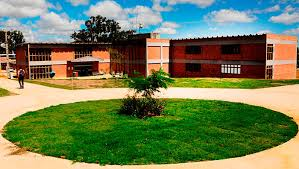
\includegraphics{images/ufape.jpeg}
\end{figure}

Perceba que, ao me referir a uma figura ou tabela específica, trato a figura ou tabela como nome próprio e utilizo letra maiúscula. Isto vale tanto para a Tabela \ref{tab:exemplo} quanto para a Figura \ref{fig:foto}. Mas se falo sem apontar o número utilizo letra minúscula para me referir àquela tabela ou a esta figura.

O mesmo vale para equações. Quando me referir a uma equação importante devo utilizar seu número. Por exemplo, a Equação \ref{eq:segundo_grau} é uma equação do segundo grau:
\begin{equation}
f(x) = ax^2 + bx + c,
\label{eq:segundo_grau}
\end{equation}
esta equação associa um função $f$ de $x$ com um polinômio do segundo grau. $a$, $b$ e $c$, são constantes que dão o peso de cada parte da equação. $a$ indica a contribuição de $x^2$, $b$ a contribuição de $x$ e, finalmente, $c$ é uma contante somada ao todo (pode ser interpretada como contribuição do 1).
Cada equação deve ser descrita, explicando o que é cada elemento dela.
Veja que a equação termina com um vírgula (poderia terminar com um ponto final). Deve-se utilizar a pontuação na equação como se ela fosse uma palavra do texto.

\section{Discussão}
A discussão pode vir na junto dos resultados, separado ou ambos (uma parte com os resultados e outra depois). A discussão é uma interpretação dos resultados, uma ``tradução''. É preciso deixar claro quais são os resultados. 
Na discussão também comparar seus resultados com os resultados de outros autores. As possibilidades são inúmeras e vai depender da sua análise.

\section{Considerações Finais}
Faça uma recapitulação do que foi visto neste capítulo. E termine fazendo uma conexão com o que será visto no capítulo seguinte.
%CAP. 5
\chapter{Conclusão}

Comece fazendo um resumo dos resultados alcançados. Diferentemente do Abstract e do Capítulo 1. Agora você pode fazer um resumo mais ``técnico'' utilizando todo o conhecimento descrito no TCC. 

Deixe claro quais os méritos do seu trabalho.

Descreva como foram alcançados os objetivos descritos no Capítulo 1. Começando pelos objetivos específicos e finalizando com o objetivo geral.

\section{Contribuições}
Destaque quais a novidades que seu trabalho trouxe, o que é original.

\section{Trabalhos Futuros}
Descreva as várias continuações que você poderia ter do seu trabalho.

% References
\begin{references}
  \bibliography{references}
\end{references}

% Appendix

% \theappendix
% \include{appendix/mapping-study}

\end{document}
